\documentclass{article}
\usepackage[utf8]{inputenc}
\usepackage{amsmath, amssymb}
\title{Compendio Lezioni del Corso: Geometria_2}
\date{\today}
\author{Federico De Sisti}
\begin{document}
\maketitle
\maketitle
	\newpage
	\section{Informazioni pratiche}
	Giovedì esercitazioni\\
	Ci sono gli esercizi settimanali! Alcuni di questi sono da sapere per l'orale\\
	Se vogliamo essere avvertiti per urgenze possiamo mandare una mail\\
	C'è il sito del corso\\
	Per la maggior parte del corso di studia su Topologia di Marco Manetti\\
	\textbf{Esami:}\\
	Ci sono 2 esoneri\\
	L'esame è scritto e orale\\
	\textbf{Prerequisiti}\\
	1) Familiarità con le funzioni continue\\
	2) Un po' di teoria dei gruppi\\
	3) Derivate di applicazioni in più variabili\\[10px]
	Il corso è diviso in 3 parti:\\
	1)Topologia generale\\
	2) Topologia algebrica\\
	3) Geometria differenziale\\
	\section{Topologia Generale}
	\subsection{Introduzione}
	Nasce per studiare sottoinsiemi di $\R^n$, cosa posso fare con un sottoinsieme di  $R^n$ con un applicazione continua?\\
	Studieremo:\\
	1) Proprietà dei sottoinsiemi di $\R^n$, come ad esempio la compattezza, da un punto di vista astratto.\\
	2) Applicheremo le stesse proprietà ad insiemi dotati di "geometria" meno intuitiva\\
	Ad esempio la topologia generale si applica in 
	\begin{itemize}
		\item Analisi
		\item Algebra
		\item Logica
	\end{itemize}
	\textbf{Esempio}\\
	In $\R^2$ prendiamo \\
	 \[
		 X = \R\times\{0,1\}
	.\] 
	%TODO inserisci grafico delle rette parallele all'asse x passanti per 00 e 01\\
	Poniamo, in maniera informale, questa relazione d'equivalenza:
	\[
		(x,0)\sim (x,1) \ \ \ \ \forall x\in\R
	.\] 
	Il quoziente "assomiglia" ad una sola retta, gli elementi equivalenti vengono "appiccicati".\\
Seconda relazione d'equivalenza:
\[
	(x,0)\sim(x,1) \text{   solo per   } x\leq 0
.\] 
$X/\sim$ in questo caso assomiglia a :\\
%TODO aggiungi immagine diapasol
Terza relazione d'equivalenza:
\[
	(x,0)\sim (x,1) \text{    solo per    } x < 0
.\] 
%TODO aggiungi immagine pisello (due punti nello stesso posto)
Una specie di analogo della figura precedente, ma il punto $[0,0]$ è raddoppiato
\begin{defi}[Funzioni continue]
	Dati $X\subseteq \R^n$ e  $Y\subseteq \R^m$ insiemi qualsiasi, si definisce continua un'applicazione  $f:X \rightarrow Y$ se 
	\[
		\forall p\in X \ \ \forall \epsilon >0\ \ \exists\delta>0\ \  \text {se} \ \ x\in X\ \  \text {soddisfa}
	.\] 
	\[
		||x-p||<\delta \ \ \text{allora} \ \ ||f(x)-f(p)||<\epsilon
	.\] 
\end{defi}
\begin{defi}[Omeomofrismo]
	Data $f: X \rightarrow Y$ si dice omeomorfismo se è biettiva, continua,\\ e $f^{-1} :Y \rightarrow X$ è continua.
\end{defi}
\textbf{Osservazione}\\
In topologia generale gli omeomorfismo hanno un ruolo analogo agli isomorfismi in algebra e algebra lineare.\\
\textbf{Esempio:}\\
1) $[0,1]$ (in  $\R$) è omeomorfo ad $[a,b] \ \ \forall a,b\in \R$ con $a<b$\\
ad esempio\\
\begin{center}
\begin{aligned}
	f:[0,1] \rightarrow [a,b]\\
	  &t \rightarrow (1-t)a + tb
\end{aligned}
\end{center}
è biettiva, continua e $f^{-1}$ è continua.\\
2) $S^1 = \{(x,y)\in \R^2|x^2 + y^2 = 1 \}$ e $Q = \{(x,y)\in\R^2 | max\{|x|,|y|\} = 1\}$\\
%TODO inserisci immagine quadrato
Per esempio possiamo normalizzare i punti del quadrato
\begin{center}
\begin{aligend}
	&Q \rightarrow S^1\\
	&p \rightarrow\frac {p}{||p||}
\end{aligend}
\end{center}
che è continua, biettiva e ha inversa continua.\\
3)$[0,1]\cup]2,3]$ non è omeomorfo a  $[0,2]$\\
ad esempio \\\begin{aligned}
	f:[0,1]&\cup]2,3] \rightarrow[0,2] \\
	&x \rightarrow \begin{cases}
		x \ \ \ \ \text{se} \ x\leq 1\\
		x - 1 \ \ \text{ se} \ x> 1
	\end{cases}
\end{aligned}\\
Con l'analisi matematica si dimostra facilmente che non esiste alcuna biezione con inversa continua.\\
\textbf{Osservazione}\\
In algebra se $f$ è un omomorfismo biettivo allora $f^{-1}$ è un omomorfismo.\\
In topologia se $f$ è continua e biettiva, $f^{-1}$ non è sempre continua.\\
4) $]0,1[$ è omeomorfo a $]a,b[$  $\forall a,b\in\R$  $a < b$\\
Inoltre  $]0,1[$ è omeomorfo a $]0,+\infty[$\\
ad esempio tramite\\
 \begin{aligned}
	 ]0,&+\infty[ \rightarrow ]0,1[\\
	    & x \rightarrow e^{-x}
\end{aligned}\\
5)$]0,+\infty[$ è omeomorfo a $\R$, ad esempio tramite $ x \rightarrow log(x)$\\
6) $]0,1[$ non è omeomorfo a $[0,1]$\\
7) $S^n = \{p\in\R^{n+1} |\ \  ||p|| = 1\}$\\
$S^n\setminus\{(0,\ldots,0,1)\}$ è omeomorfo a $\R^n$
%TODO inserisci disegno circonferenza senza un punto
Ad esempio tramite la proiezione stereografica (esercizio: vedere la formula)\\
8) Ci sono molti esempi di figure omeomorfe fra loro, ma un omeomorfismo esplicito è difficile, ad esempio.\\
un $l$-agono regolare qualsiasi (in  $\R^n$) e un  $r$-agono qualsiasi sono omeomorfi ($\forall\ l,r\geq 3)$ \\
9)  $\R^n$ e $\R^m$ sono omeomorfi se e solo se  $n = m$ (è un teorema difficile, nel corso vedremo la dimostrazione per qualche esponente specifico, $n\leq 2$)\\
Vediamo due riformulazioni della continuità.
\begin{defi}
$A\subseteq \R^n$ si dice aperto se 
\[
	\forall p\in A \ \ \exitst \varepsilon > 0 \ \ | \ \ \text{se}\ \  x\in \R^n
.\] 
\[
	\text{soddisfa } \  ||x-p|| <\espilon \ \text{ allora } x\in A
.\] 
\end{defi}
\begin{nota}
	$B_\varepsilon (p) = \{x\in\R^n| \ ||x-p|| < \epsilon\}$\\
	è la palla aperta di centro $p$ e raggio $\varespilon$
\end{nota}
\begin{defi}
	Sia $X\subseteq \R^n$ e  $p\in \R^n$ p si dice aderente a $X$ se  $\forall \espilon>0 \ \exists x\in X \  | \ ||x-p||<\epsilon$
	%TODO aggiungi disegno palla storta 
	(chiaramente se $p\ini X$  allora è aderente a $X$, basta prendere  $x = p$)
\end{defi}
\textbf{Esempio:}\\
$1\in\R$ è aderente a $X = [0,1[$\\
 \begin{prop}
	Sia $f:\R^n \rightarrow\R^m$ Sono equivalenti:
	\begin{enumerate}
		\item $f$ è continua
		\item $\forall Z\subseteq \R^n \ \ \forall p\in \R^n$ se $p$ è aderente a $Z$\\ allora  $f(p)$ è aderente a $f(Z)$ 
		\item $\forall A\subseteq \R^m$ se  $A$ è aperto, allora $f^{-1}(A)$ è aperto.
	\end{enumerate}
\end{prop}
\begin{dimo}
	$1) \Rightarrow  2)$ \\
	Siano $Z\subseteq\R^n, p\in\R^n$ suppongo $p$ aderente a  $Z$, dimostriamo che  $f(p)$ è aderente a $f(Z)$\\
	%TODO aggiungi immagine palla in quadrato
	Sia  $\epsilon > 0 $ qualsiasi, sia $\delta > 0 $, dalla continuità di  $f$ in $p$. Dato che $p$ è aderente a $Z$ esiste  $z\in Z$  tale che  $||z-p|| < \delta$.\\
	Allora  $f(z)$ è un punto di $f(Z)$ e  $||f(p)-f(z)|| < \varepsilon$.\\
	 $2) \Rightarrow 3)$ \\
	 Sia $A\subseteq \R^m$ aperto, dimostriamo che $f^{-1}(A)$ è aperto, dimostriamo che $f^{-1}(A)$ è aperto in $\R^m$\\
	 %TODO aggiungi immagine\\
	 Sia  $p\in f^{-1}(A)$ sia $f(p)\in A$\\
	 Per assurdo supponiamo.\\
	 $\forall \varespilon > 0 \exists q\in\R^n$ fuori da  $f^{-1}(A)$ ma  $||p-q|| < \varepsilon$.\\
	 Allora $p$ è aderente a  $\R^m\setminus f^{-1}(A)$.\\
	 Segue, per 2),  $f(p)$ è aderente a $f(\R^n\setminus f^{-1}(A))$\\
	 quindi per ogni  $\eta > 0$ esistono punti a distanza  $< \eta$ non in  $f(\R^n\setminus f^{-1}(A))$ punti che non vanno in $A$\\
	 allora  $f(p)$ è aderente a $\R^m\setminus A$. Questo è assurdo perché  $A$ è aperto\\
	 La terza implicazione la vediamo lunedì
\end{dimo}

% -------------------- Fine Lezione 1 --------------------

\maketitle
	\newpage
	\section{Spazi Topologici}
	\begin{defi}[Topologia]
		Sia $X$ un insieme, $T\subset P(X)$\\
		 $T$ è detta Topologia se:
		 \begin{enumerate}
			 \item $X,\emptyset\in T$
			 \item Unione di una famiglia qualsiasi di elementi in  $T$ è un elemento di $T$ 
			 \item intersezione di 2 elementi qualsiasi di $T$ è un elemento di $T$.
		 \end{enumerate}
		 In tal caso gli elementi di $T$ sono detti aperti di $T$.\\
		 La coppia $(X,T)$ è detta \textbf{spazio topologico} (o anche semplicemente insieme $X$)
	\end{defi}
	\textbf{Osservazione}
	\begin{itemize}
		\item Famiglia qualsiasi vuol dire infinita numerabile, o finita, o non numerabile, o anche vuota
		\item L'intersezione di una famiglia finita di elementi di $T$ è ancora un elemento di $T$ 
		\item Possiamo interscambiare la precedente affermazione e la proprietà 3 della definizione
	\end{itemize}
	\textbf{Nota}
	\begin{itemize}
		\item "intervallo aperto" = $]a,b[\subseteq\R$ come al solito
		\item aperto = elemento della topologia $T$
	\end{itemize}
	\textbf{Esempi}
	1) Ogni insieme è dotato almeno delle seguenti topologia
	\begin{enumerate}
		\item $T = \{X,\emptyset\}$, detta \textbf{topologia banale}
		\item $T = P(x)$, detta \textbf{topologia discreta}
	\end{enumerate}
	Osserviamo che, nella topologia discreta, $\{x\}$ è aperto $\forall x\in X$\\
	2)  $X = \R^n$\\
	$T = \{ A\subseteq X \ | \ \forall a\in A \ \exists \varepsilon > 0 \ t.c. \ B_\varepsilon(a)\subseteq A\}$ è la topologia euclidea\\
	La dimostrazione del fatto che sia una topologia è un esercizio per casa\\
	3) Sia $X$ insieme, $p\in X$. Definiamo  $T = \{A\subseteq X \ | \ p\in A, $ oppure $A = \emptyset\}$  $T$ è una topologia\\
	4) $X$ insieme, poniamo $T = \{A\subseteq X \ | \ X\setminus A $ è finito, oppure $A = \emptyset\}$\\
$T$ è una topologia, detta \textbf{topologia cofinita}\\
\begin{defi}
	Sia $(X,T)$ spazio topologico, $C\subseteq X$ è chiuso se $X\setminus C$ è aperto 
\end{defi}
\begin{lemm}[Proprietà degli insiemi chiusi]
Per gli insiemi chiusi di qualunque topologia valgono:
	\begin{enumerate}
		\item $X,\emptyset$ sono chiusi
		\item intersezione di una famiglia qualsiasi di chiusi è un chiuso
		\item Unione finita di chiusi è un chiuso
	\end{enumerate}
\end{lemm}
\begin{dimo}
	1. ovvio\\
	2. $\displaystyle x\setminus \left( \bigcap_{i\in I}C_i \right) = \bigcup^{i\in I}_{X\setminus C_i}$ che è unione di aperti\\
	3. $(X\setminus(C\cup D)) = (X\setminus C)\cap (X\setminus D)$ che è intersezione di 2 aperti.
\end{dimo}
\textbf{Osservazione}\\
In uno spazio topologico ci sono insiemi sia aperti che chiusi (clopen = closed + open)\\
\textbf{Esempio}\\
$X = \R$\\ 
Il sottoinsieme  $[0,1]$ è chiuso in topologia euclidea\\
è chiuso e aperto in topologia discreta\\
non è chiuso in topologia banale\\
non è chiuso in topologia cofinita, e neanche aperto\\
\begin{defi}
	Sia $X$ spazio topologico con topologia $T$. Sia $B\subseteq T$  $B$ è detta base se ogni aperto si può scrivere come unione di elementi di $B$
\end{defi}
\textbf{Esempi}
\begin{enumerate}
	\item Sia $T$ topologia su $X, \Rightarrow B=T$ è una base
	\item Sia $T$ topologia discreta su $X, B = \{\{x\} \ | \ x\in X\}$  è una base di $T$
	\item Sia  $X = \R$, $T = $ topologia euclidea. $B = \{]a,b[ | a < b \in \R\}$ è una base di  $T$\\
		Infatti  $B\subseteq T$ perché $]a,b[$ è aperto in topologia euclidea. Inoltre ogni aperto si può scrivere come unione di elementi di $B$\\
		 \begin{dimo}
			Sia $A\in T$ euclidea su $\R$\\
			$ \Rightarrow \forall p\in A\ \ \ \exists \varepsilon > 0 $ t.c. \ \ $]p-\varepsilon, p + \varepsilon[ \subseteq A$\\
			$ \Rightarrow A = \bigcup_{p\in A} ]p-\varepsilon, p + \varepsilon[\ \in B$
		\end{dimo}
\end{enumerate}
\textbf{Osservazione}\\
Data $B$ base di $T$ topologia, la topologia $T$ è determinata da $B$ Infatti:
\[
	T = \{\text { unione arbitraria di elementi di } B\}
.\] 
\begin{prop}
	Sia $X$ insieme, $B\subseteq P(X)$ famiglia di sottoinsiemi di  $X$. Esiste $T$ topologia t.c. $B$ è sua base se e solo se
	\begin{enumerate}
		\item $X$ è unione di elementi di $B$
		\item  $\forall A,A'\in B, A\cap A'$ è unione di elementi di $B$
	\end{enumerate}
\end{prop}
\begin{dimo}
	$( \Rightarrow )$ \\
	$\exists T$ topologia di cui $B$ è base (per ipotesi)\\
	\begin{itemize}
		\item $ \Rightarrow $ $X\in T$ e $B$ è base di $T \Rightarrow $ (1) vera
\item $ \Rightarrow A$ e $A'\in T \Rightarrow A\cap A'\in T \Rightarrow $ (2) vera
	\end{itemize}
	$ ( \Leftarrow )$ \\
	Definisco $T = $ unioni arbitrarie di elementi di $B$ e verifico che sia una topologia
	\begin{itemize}
		\item $X\in T, \emptyset\in T \Rightarrow $ (1) vera ($\emptyset\in T$ perché $\emptyset = \emptyset\cup\emptyset\cup\ldots )$
		\item Per costruzione di  $T$, unioni di elementi di $T$ sono elementi di $T\ \Rightarrow \ $ (3) vera
		\item $D,E\in T \Rightarrow D = \bigcup_{i\in I} A_i, E = \bigcup_{i\in J}A'_j, \ \ A_i,A'_j\in B \  \ \forall i,j$ \\
			$ \Rightarrow D\cap E = \bigcup^{}_{i\in I, j\in J}(A_i\cap A'_j)$
	\end{itemize}
	\textbf{Osservazione:}\\
	Ciascuno $A_i\cap A'_j$ è unione di elementi di $B.$ \\
	$ \Rightarrow D\cap E$ è unione di elementi di $B$\\
	 $ \Rightarrow T $ è topologia (e $B$ sua base per costruzione)
\end{dimo}
\textbf{Osservazione}\\
La proprietà (2) è equivalente a:
\[
	\forall A,A'\in B, \ \ \forall p\in A\cap A' \ \exists D\in B \ \text{ t.c } p\in D\subseteq A\cap A'
.\] 
\textbf{Esempio}\\
Sia $\mathbb \mathbb{K}$ un campo, consideriamo $x = \mathbb \K^n$, Dato  $f\in \mathbb K[x_1,\ldots,x_n]$\\
Poniamo $x_f = \{p\in\mathbb K^n \ | \ f(p)\neq 0\}$\\
$ \Rightarrow  B = \{x_f \ | \ f\in \mathbb K[x_1,\ldots,x_n]\}$ \\
(esempio: $x = \r, n = 1, \mathbb k = \r, \ f(x) = (x-1)(x-2) \leadsto x_f= \R\setminus\{1,2\}$)
(esempio: $X = \R, n = 2, \mathbb K = \R^2, \ f(x,y) = x^2 + y^2 - 1, x_f = \R^2\setminus S^1)\\$
Allora $B$ è base di una topologia $T$ su $X$\\
Verifichiamo usando la proposizione precedente\\
 $X = X_f, f = 1$ polinomio costante, allora (1) ok\\
 Prendiamo $A, A'\in B$ studiamo $A\cap A'$\\
 $A = x_f, \ A'=x_g$ con $f,g \in \mathbb K[x_1,\ldots,x_n]$, Allora\\
 $A\cap A' = X_{fg}$ è essa stessa un elemento di $B$ quindi (2) ok \\
 per la proposizione precedente $ \Rightarrow \exists$ topologia $T$\\
 La topologia così definita è detta la topologia di Zariski in  $\mathbb K^n$
	\textbf{Esempio}\\
	$\K = \R, n = 1$\\
	$\R\setminus\{1,2\}$ è aperto in topologia euclidea e in topologia di Zariski.\\
	$[0,1]\subseteq\R$ è chiuso in topologia euclidea, è chiuso in topologia di zariski? Esercizio per casa\\

	\begin{defi}
		$T_1,T_2$ topologie su $X$, $T_1$ è detta più fine di $T_2$ se $T_2\subseteq T_1$
	\end{defi}
	\textbf{Osservazione}\\
	Prese 2 topologie a caso, non è detto che siano confrontabili.\\
	\textbf{Esempio}\\
	La topologia banale è la meno fine di tutte, Quella discreta è la più fine.\\
	\begin{propo}
		Siano $ T_1,T_2$ topologie su $X$. Allora\\
		$T_1\cap T_2$ è una topologia.\\
		Inoltre $T = T_1\cap T_2$ è meno fine di $T_1$ e meno fine di $T_2$
	\end{propo}
	\begin{dimo}
		Esercizio lasciato al lettore
	\end{dimo}

% -------------------- Fine Lezione 2 --------------------

\maketitle
	\newpage
	\subsection{Parte interna, chiusura,intorni}
	\begin{defi}
		Sia $X$ spazio topologico, sia $D\subseteq X$ un sottoinsieme, la parte interna di  $D$ è 
		\[
		 D^o = \bigcup_{A\subseteq D, A\text{ aperto } } A
		.\] 
		La chiusura di $D$ è 
		\[
			\overline D = \bigcap_{C\supseteq D, C \text{ chiuso}} C
		.\] 
		la frontiera di $D$ è
		\[
		 \partial D = \overline D \setminus D^o
		.\] 
		I punti di $D^o$ si dicono interni a $D$, quelli di $\overline D$ si chiamano aderenti a $D$.
	\end{defi}
	\textbf{Osservazioni}\\
	1) $D^o$ è un aperto e  $\overline D$ è un chiuso (posso vederlo come l'intersezione tra  $\overline D$ e il complementare di $D^o$, che è chiuso)\\
	 2) Anche $\partial D$ è chiuso perché\\
	 $\parial D = \overline D\cap (X\setminus D^o)$ dove  $(X\setminus D^o)$ è un chiuso\\
	  \textbf{Esempio}\\
	  1) $X = \R$ con topologia euclidea. Sia $D = [0,1]$.\\
	  Allora  $D^o = ]0,1[$, verifica:\\
	  $D^o \supseteq ]0,1[: $\\
	  La parte interna di  $D$ contiene tutti gli aperti, dato che  $]0,1[$ è un aperto è contenuto.\\A
	  $D^o\subseteq ]0,1[$:\\
	  supponiamo per assurdo che  $D^o\not \subseteq ]0,1[$ , allora $0\in D^o$ oppure  $1\in D^o$ ( mi limito a considerare i punti di  $D$ perché $D^o\subseteq D$).\\
	  Supponiamo  $0\in D^o$, allora esiste  $A\subseteq \R$ aperto t.c.  $A\subseteq D, A\ni 0$ (è uno degli A della definizione).\\
	  Allora  esiste $\varepsilon > 0$ t.c.  $]0 - \varepsilon , 0 + \varepsilon[\subseteq a \subseteq D$.\\
	  assurdo, Analogamente  $1\not\in D^o$ quindi vale  $\subseteq$\\
	  2)  $X = \R$ con topologia cofinita $D = [0,1]$. Allora  $D^o = \bigcup_{A\subseteq D, A \text{ aperto}}$ \\
	  Sia  $A$ aperto.\\
	  $A\subseteq D$ abbiamo\\
	  $A = \emptyset $ oppure $A = \R\setminus\{\text{insieme finito}\}$\\
	  Ma questa ultima è impossibile\\
	  allora  $D^o = \emptyset$ in questa topologia (con questo $D$)\\
	  esercizio: calcolare $\overline D$\\
	  3)  $X = \R$, $T = $ topologia per cui $A$ è aperto $ \Leftrightarrow A = \emptyset$ oppure $A\ni 0$ \\
	  Considero $\overline{\{1\}} = \{1\}$, questo insieme non contiene lo zero, quindi $\{1\}$ è esso stesso un chiuso.\\
	  Però $\overline{\{0\}} = ?$ \\
	  I chiusi in  $T$ sono $\R$ e i sottoinsiemi che non contengono lo  $0$. Quindi l'unico insieme chiuso che contiene $\{0\}$ è $\R$, allora $\overline{\{0\}} = \R$
	   \begin{defi}
	  	Sia $X$ spazio topologico, un sottoinsieme di $D\subseteq X$ si dice denso se $\overline D = X$
	  \end{defi}
	  \textbf{Esempio}\\
	  $X = \R $ con topologia euclidea,\\
	  $D = \Q$. Dimostriamo che è denso\\
	  L'unico chiuso che contiene  $D$ è $X$ stesso.\\
	   Sia $C\subseteq \R$ chiuso con  $C\supseteq \Q$\\
	   sia $a\in\R\setminus C$ aperto\\
	   allora  $\exists \varepsilon > 0 \ | \ ]a - \varepsilon, a + \varepsilon[ \subseteq \R\setminus C$ \\
	   allora $] a - \varepsilon, a + \varepsilon[\cap \Q = \emptyset$ \\
	   assurdo.\\
	   Allora $a$ non esiste e $C = \R$. 
	   \textbf{Osservazione:}\\
	   1) Sia  $D\subseteq X$ spazio topologico\\
	   vale:\\
	    \[
	   X\setminus(\overline D) = (X\setminus D)^o
	   .\] 
	   \begin{dimo}
	   	Usando direttamente la definizione:\\
		\[
			X\setminus(\overline D) = X\setminus (\bigcap_{C\supseteq D, C \text { chiuso}}C) = \bigcup_{C\supset D, C \text { chiuso}}(X\setminus C) 
		.\] 
		(ultima eguaglianza per esercizio)
		\[
			= \bigcup_{A = X\setminus C, C\supset D, C\text{ chiuso}}A = \bigcup_{A\text{ aperto}, X\setminus A\supset D} A= \bigcup_{A\text{ aperto}, A\subseteq X\setminus D}A
		.\] 
	   \end{dimo}
	   2) $D$ denso\\
	   $\text{}\ \ \ \ \ \ \ \ \ \ \ \ \ \storto \Leftrightarrow$\\
	   $D$ interseca ogni aperto non vuoto (esercizio)
	   \begin{defi}
	   	Sia $X$ spazio topologico,\\
		$U\subseteq X, x\in U^o$\\
		Allora  $U$ si dice intorno di $x$.\\
		Equivalentemente, un sottoinsieme $U\subseteq X$ si dice intorno di $x\in X$ se esiste  $A\subseteq X$ aperto t.c. $x\in A\subseteq U$
	   \end{defi}
	   \textbf{Esempio}\\
	   $X = \R$ topologia euclidea,  $x = 0, U = ]-1,1[$ è intorno di  $x$ (si prende ad esempio $A = U, $ o anche $A = ]-1/2,1/2[$\\
	   Anche $V = [-1,1]\cup \{5\}$ è un intonro di 0, ad esempio  $A = ]-1/2, 1\16[\cup]3/16,7/16[$\\
	    \textbf{Osservazione}\\
	    $U\subseteq X$ è aperto  $ \Leftrightarrow U = U^o \Leftrightarrow U$ è  un intorno di ogni suo punto.
	    \begin{lemm}
Siano $X$ spazio topologico, $x\in X$ $D\subseteq X.$ Allora $x\in\overline D \Leftrightarrow \forall U$ intorno di $x$ vale $U\cap X \neq\emptyset$
	    \end{lemm}
	    \begin{dimo}
	    Supponiamo $x\in\overline D$ sia $U$ intorno di $x$\\
	    per assurdo suppongo  $D\cap U = \emptyset$
	    %TODO se vuoi aggiungi foto marzo 4 6:27
	    Considero  $A  \subseteq X$ aperto con $x\in A\subseteq U$\\
	    Considero il chiuso  $X\setminus A = C$\\
	    Abbiamo  $C\supseteq D$ perché  $D\cap U = \emptyset$ e allora anche $D\cap A = \emptyset$A\\
	    Abbiamo  $C\supset D$ perché  $D\cap U = \emptyset$ e allora anche  $D\cap A = \emptyset $ e allora anche $D\cap A = \emptyset$. Cioè $C$ compare nella definizione di $\overliene D $ e $C\not\ni x$ perché  $x\in A$\\
	    Ma  $x\in\overline D$ quindi  $x$ è in tutti i chiusi che contengono $D$, assurdo\\
	    Viceversa, supponiamo $D$ intorno di $x$, per assurdo però $x\neq \overline D$, Allora esiste un chiuso  $C$ che contiene $D$ ma non $x$.\\
	    Considero  $A = X\setminus C$ è un aperto contenente  $x$. Cioè $A$ è un intorno di $x$ e $A$ non interseca $D$; assurdo. Quindi $x\in D$ 
	    %TODO se vuoi aggiungi immaigne 4 mar 6:36
	    \end{dimo}
	    \begin{defi}[Famiglia degli intorni, sistema fondamentale]
	    	Sia $X$ spazio topologico e $x\in X$ La famiglia di tutti gli intorni di  $x$ si denota con $I(x)$.\\
		Un sottoinsieme $J\subseteq I(x)$ è detto sistema fondamentale di intorni di $x$ (o base locale in $x$) se $\forall U\in I(x)\ \  \exists V\in J \ |\ V\subseteq U $ 
	    \end{defi}
	    \textbf{Esempi:}\\
	    $X = \R$ con topologia euclidea.\\
	     $x\in\R$ qualsiasi\\
	     $J = \{]x - \varepsilon, x+ \varepsilon[ \ |\ \varepsilon > 0,  \ \varepsilon \in\R\} $\\
	     è sistema fondamentale di intorni di  $x$\\
	     $J'\{[x- \frac 1n, x + \frac 1n] \ | \ n\geq 1, \  n\in\N\}$ \\
	     è un sistema fondamentale di interni di $x$\\
	     \[
		      J''= \{[x-\frac 1n, x + \frac 2n[\cup \{x + \frac 3n \} | n\geq 1, n\in\N\}\\
	     .\] 
	     è un sistema fondamentale di riferimento
	      \[
		      J'''= \{]x-\frac 1n, x + \frac 1n[\cup \{10 \} | n\geq 1, n\in\N\}\\
	     .\] 
	     $(10\neq x)$\\
	     non è un sistema fondamentale di riferimento\\
	     \subsection{Applicazioni continue}
	     \begin{defi}
		     Siamo $X, Y$ spazio topologico $f : X \rightarrow Y$ un'applicazione. $f$ si dice continua se $f^{-1} (A)$ è aperto (in $X$) $\forall A$ aperto ($Y$)
	     \end{defi}
	     \textbf{Nota (per la tesi)}\\
	     non iniziare mai una frase con un simbolo, è facile fare errori  (lui può ma solo per essere veloce)\\
	     \textbf{Esempi:}\\
	     1) Se $X$ ha topologia discreta, ogni $f$ è continua (qualsiasi sia $Y$)\\
	     2) Se  $Y$ ha una topologia banale, allora $f^{-1}(\emptyset) =\emptyset, f^{-1}(Y) = X$\\
	     quindi ogni $f$ è continua.\\
	     3) Supponiamo $X,Y$ con topologia cofinita e $f:X \rightarrow Y$ iniettiva\\
	     $f^{-1}(\emptyset) = \emptyset, \ $\\
	     gli altri aperti sono del tipo $Y\setminus\{$ insieme finito  $\} = Y\setminus\{y_1,\ldots, y_n\}$\\
	     allora:\\
	     $f^{-1}(Y\setminus\{y_1,\ldots,y_n\}) = X\setminus\{f^{-1}(y_1)\cup\ldots\cup f^{-1}(y_n)\}$
	     e tutte le controimmagini di questi elementi sono o vuote o di cardinalità 1, quindi è aperto.

% -------------------- Fine Lezione 3 --------------------

\maketitle
	\newpage
	\section{Prima lezione di esercizi}
	mail del tipo degli esercizi: zenobi@altamatematica.it
	\[
	 D^2 = \{(x,y)\in\R^2 | \sqrt {x^2 + y^2 }\leq 1\}
	.\] 
	\[
		Q = \{(x,y)\in\R^2 | |x|\leq 1, |y|\leq 1\} = [0,1]\times[0,1]
	.\] 
	Esempio

% -------------------- Fine Lezione 4 --------------------

\maketitle
	\newpage
	\subsection{Funzioni continue}
	\textbf{Osservazione}\\
	Siano $X,Y$ spazi topologici, $f: X \rightarrow Y$.\\
	Siano $A\subseteq Y$ un sottoinsieme,
	 \[
		 X\setminus f^{-1}(A) = \{x\in X \ | \ f(x)\not\in A\} = \{x\in X | f(x) \in Y\setminus A\} = f^{-1}(Y\setminus A)
	.\] 
	Analogamente, con $A,B\subseteq Y$ e $C,D\subseteq X$
	\[
	 f^{-1}(A\cup B) = f^{-1}(A)\cup f^{-1}(B)
	.\] 
	\[
	f^{-1}(A\cap B) = f^{-1}(A)\cap f^{-1}(B)
	.\] 
	\[
	 f(C\cup D) \neq f(C)\cup f(D)
	.\] 
	\[
	 f^{-1}(f(C))\supsetneq C
	.\] 
	\[
	 f(f^{-1}(A)) = A\cap Im(f)
	.\] 
	Tornando a $f: X \rightarrow Y$\\
	$f$ continua $ \Leftrightarrow f^{-1}(A)$ aperto $\forall A\subseteq Y$ aperto $ \Leftrightarrow X\setminus f^{-1}(A) = f^{-1}(Y\setminus A) $ chiuso \ \ $\froall A\subseteq Y$ aperto $ \Leftrightarrow$ con $C = Y\setminus A$ $f^{-1}(C)$ chiuso $\forall C\subseteq Y$ chiuso.
	\begin{defi}[Continuità]
		Sia $f:X \rightarrow Y$ applicazione fra spazi topologici. Sia $p\in X$,  $f$ è continua in $p$ se
		\[
			\forall U\subseteq Y\text{ intorno di } f(p) \ \exists V\subseteq X \text{ intorno di } p \text{ t.c } f(V)\subseteq U
		.\] 
	\end{defi}

	\begin{teo}
		Sia $f:X \rightarrow Y$ applicazione fra spazi topologici, sono equivalenti:
\begin{enumerate}
	\item $\forall p\in X:\  f$  è continua in $p$
	\item  $\forall Z\subseteq X: \ f(\bar Z)\subseteq \overline {f(X)}$  
	\item $f$ continua
\end{enumerate}
	\end{teo}
	\begin{dimo}
		$1) \Rightarrow 2)$ Sia $p\in \overline Z$ so che  $f$ è continua in $p$.\\
		Voglio dimostrare che 
		 \[
		 f(p)\in \overline{f(Z)}
		.\] 
		Formuliamo questa condizione in termini di intorni:\\
		devo dimostrare che in ogni intorno di $f(p)$ ci sono punti di  $f(Z)$. Sia $U\subseteq Y$ intorno di  $f(p)$ per continuità in $p$ $\exists V\subseteq X$intorno di  $p$ tale che $f(V)\subseteq V$ \\
		Visto che $p\in \overline Z$ esiste  $z\in Z$ tale che $z\in V$\\
		Allora  $f(z)$ è in $U$ e in $f(Z)$\\
		cioè ogni intorno $U$ di $f(p)$ contenente punti di $f(Z),$ cioè $f(p)\in \overline{f(Z)}$\\[10px]
		$2) \Rightarrow 3)$ Dimostriamo che $f^{-1}(C)$\\
		è chiuso  $\forall C\subseteq Y$ chiuso. Considero $f^{-1} (C)$, voglio dimostrare che è chiuso confrontandolo con  $\overline{f^{-1}(C)}$.\\
		L'ipotesi 2) dice:
		 \[
			 f(\overline{f^{-1}(C)})\subseteq\overline{f(f^{-1}(C))} = \overline{C\cap f(X)}\subseteq C
		.\] 
		Dato che $C$ è un chiuso che contiene $C\cap f(X)$\\
		Allora  $\overline{f^{-1}(C)}\subseteq f^{-1}(C)$\\
		D'altronde vale sempre  $\overline{f^{-1}(C)} \supseteq f^{-1}(C)$\\
		quindi  $\overline{f^{-1}(C)}= f^{-1}(C)$\\
		da cui  $f^{-1}(C)$ è chiuso.\\[10px]
		$3) \Rightarrow 1)$ suppongo $f$ continua, sia $p\in X$, sia $U\subseteq Y$ intorno di $f(p)$ scegliamo $a\subseteq Y$ aperto con $f(p)\in A \subseteq U$\\
		per continuità:
		$f^{-1}(A)$ aperto di $X$ e contiene  $p$,\\
		posso prendere  $V = f^{-1}(A)$, intorno aperto di $p$, ed è tale che  $f(V)\subseteq A\subseteq U$\\
	\end{dimo}
	\begin{prop}
		La composizione di applicazioni continue qualsiasi è continua
	\end{prop}
	\begin{dimo}
		Siano $X \xrightarrow{f}{} Y \xrightarrow{g}{}Z$\\
		applicazioni fra spazi topologici, suppongo $f\circ g$ continue,\\
		dimostriamo che $g\circ f$ è continua.\\
		Sia $Z$ aperto dimostriamo che
		\[
		 (g\circ f)^{-1}(A) \text{ è aperto } 
		.\] 
		\[
			(g\circ f)^{-1}(A) = \{x\in X \ | \ (g\circ f)(x)\in A\}
		\] 
		\[
			= \{x\in X \ | \ f(x) \in g^{-1}(A)\} = f^{-1}(g^{-1}(A))
		.\] 
		$g$ manda aperti in aperti, stesso per $f$, segue che la composizione fa lo stesso.
	\end{dimo}
	\newpage
	\begin{defi}
		Siano $X,Y$ spazi topologici, $f : X \rightarrow Y$.
		\begin{enumerate}
			\item $f$ si dice omeomorfismo se $f$ è continua, biettiva, e $f^{-1}:Y \rightarrow X$ è continua
			\item $X$ e $Y$ si dicono omeomorfi se esiste $f: X  \rightarrow Y$ omeomorfismo
			\item $f$ (non necessariamente omeomorfismo, non necessariamente continua) si dice aperta se $f(A)$ è aperto $\forall A\subseteq X$ aperto, e  $f$ si dice chiusa quando $f(C)$ è chiuso $\forall C\subseteq X$ chiuso
		\end{enumerate}
	\end{defi}
	\textbf{Esempi:}\\
	$\R$ con topologia euclidea, $f : \R \rightarrow\R$ applicazione costante $f(x) = q \ \ \forall x\in \R$.\\
	Questa $f$ non è aperta, perché $\R$ è aperto in $\R$ e  $f(\R) = \{q\}$ non è aperto in topologia euclidea.\\
	\textbf{Esempio importante:}\\
	Applicazione non chiusa.\\
	\begin{aligned}
		$p : &\R^2 \rightarrow\R$\\
		$(x&,y) \rightarrow x$
	\end{aligned}\\
	$(\R^2, \R$ con topologia euclidea $)$\\
	Non è chiusa, prendiamo ad esempio  $C = \{(x,y) \ | \ x\cdot y = 1\}$\\
	è un chiuso in $\R^2$, ma $p(C) =   \R\setminus\{0\}$ non è chiuso.\\

	$C$ è chiuso di  $\R^2$ perché $C$ è uguale a $f^{-1}(\{1\})$ dove \\
	\begin{aligned}
		$f:\R^2 &\rightarrow\R$\\
		$(x,y)	& \rightarrow xy$
	\end{aligned}\\
	Infatti $f $ è continua e $\{1\}\subseteq \R$ è un chiuso.\\
	\subsection{Spazi metrici}
	\begin{defi}
		sia $X$ un insieme e $d:X\times X \rightarrow\R$\\
		$d$ si dice distanza se:
		\begin{enumerate}
			\item $d(x,y)\geq 0 \ \ \forall x,y\in X,$\\ 
				$d(x,y) = 0 \Leftrightarrow x = y$
			\item $d(x,y) = d(y,x) \ \ \forall x,y\in X$
			\item $d(x,z)\leq d(x,y) + d(y,z)$\\
				 $\forall x,y,z\in X$
		\end{enumerate}
		In tal caso $(X,d) (o X$ stesso $)$ si chiama spazio metrico
	\end{defi}
	\textbf{Esempio}\\
	Sia $X$ insieme, poniamo
	\[
	 d(x,y) = \begin{cases}
		 0 \ \ \text{ se } x = y\\
		 1 \ \ \text{ se } x \neq y
	 \end{cases}
	.\]
	$d$ è una distanza.
	\begin{defi}
		Sia $(X, d)$ spazio metrico.
		\begin{enumerate}
			\item La \underline{palla aperta} di centro $x$ e raggio $\varepsilon\in \R_{>0}$ è: \\$B_\varepsilon(x) = \{p\in X \ | \ d(p,x) < \varepsilon\}$ 
			\item La \underline{topologia indotta} da $d$ su $X$ è definita da:\\
				 $A$ aperto $ \Leftrightarrow \ \forall a\in A\ \exists \varepsilon < 0 \ | \ B_\varepsilon (a)\subseteq A$\\
				 La denotiamo con $T_d$
		\end{enumerate}
	\end{defi}
	Verifica che $T_d$ è topologia
	\begin{enumerate}
		\item $\emptyset, X$ sono aperti: ovvio
		\item unione di aperti è aperto: ovvio
		\item Siano $A_1, A_2\in T_d$, verifichiamo che $A_1\cap A_2\in T_d$, sia $a\in A_1\cap A_2$ quindi $\exists \varepsilon > 0 \ | \ B_\varepsilon (a)\subseteq A_1$ e $\exists \delta > 0 \ | \ B_\delta(a)\subseteq A_2$\\
			sia $\gamma = \min\{\varepsilon, \delta\}$ allora soddisfa  $B_\gamma (a)\subseteq A_1\cap A_2$
	\end{enumerate}
	\begin{lemm}
		Sia $(X,d)$ spazio metrico e $T_d$ la topologia indotta da $d$ 
		\begin{enumerate}
			\item $\forall p\in X \ \forall \varepsilon > 0 \ \ B_\varepsilon (p)\in T_d $
			\item $B = \{B_\varepsilon (p) \ | \ p\in X, \varepsilon \in \R_{>0}\}$\\
				è una base di  $T_d$ 
			\item Un sottoinsieme $U\subseteq X$ è intorno di $p\in X$ se e solo se \\ $\exists \varepsilon > 0 \ | B_\varepsilon(p)\subseteq U$
		\end{enumerate}
	\end{lemm}
	\begin{dimo}
		Per esercizio.
	\end{dimo}
	\textbf{Osservazione}\\
	Gli spazi metrici in generale si comportano in modo simile a $\R& n$ con distanza euclidea, ma attenzione: non tutto è uguale, ad esempio se $(X,d)$ è uno spazio metrico e $x\in X:$
	 \[
		 \{p\in X \ | \ d(x,p)\leq \varepsilon\}
	.\] 
	con $\varepsilon > 0 $ fissato, è un chiuso di $X$ (verifica per esercizio) ma non è sempre la chiusura di $B_\varepsilon (x)$.\\
	Ad esempio  $X = \R$ con distanza  $d(x,y) = \begin{cases}
		0\ \  \text{ se } x = y\\
		1 \ \ \text{ se } x\neq y
	\end{cases}$ \\
	Considero $\{p\in\R \ | \ d(p,x)\leq 1\} = \R$\\
	ma $B_1(x) = \{x\}$\\
	Questo vale  $\forall x\in \R$\\
	cioè ogni ogni singoletto è aperto, allora  $T_d$ è discreta, quindi $\{x\}$ è anche chiuso. Cioè $B_1(x) = \{x\}$.\\
	 \textbf{Osservazione:}\\
	 Siano $X,Y$ spazi metrici sia $p\in X$\\
	  $f: X \rightarrow Y$, allora $f$ è continua in $p$\\
	   $($ come applicazione fra spazi topologici, dove su $X $ e $Y$ metto le topologie indotte dalle distanze) $ \Leftrightarrow \  \forall \varepsilon > 0 \ \ \exitsts \delta > 0 \ | \ $ se $d(x,p) < \delta$ allora  $d(f(x),f(p)) < \varepsilon$\\
	   Verifica per esercizio
	   \begin{coro}
	   	Siano $d, h$ distanze su uno stesso insieme $X.$\\
		Allora  $T_d$ è più fine di $T_h$ se $\forall p\in X \ \ \forall \varepslion > 0\ \ \exists \delta > 0 \ |  \ B_\delta^d(p)\subseteq B_\varepsilon ^h(p)$
	   \end{coro}
	   \begin{dimo}
	   	Usiamo $id_X: X \rightarrow X$ dove nel dominio prendiamo $d$ e $T_d$, e nel codominio la distanza $h$ e $T_h$. Con questa scelta l'identità su $X$ è continua $ \Leftrightarrow$ $T_d\supseteq T_h$\\
		La carindalità di  $Id_X$ è equivalente alla condizione con $\varepsilon$ e $\delta$ per l'osservazione.
	   \end{dimo}
	   \begin{defi}[Distanze equivalenti]
	   	Date distanze $d,h$ su un insieme $X$, esse si dicono equivalenti se $T_d = T_h$
	   \end{defi}
	   \begin{defi}[Spazio topologico metrizzabile]
	   	Sia $X$ uno spazio topologico con topologia $T$. Se esiste una distanza $d$ su $X$ tale che $T = T_d$ allora $X$ si dice metrizzabile.
	   \end{defi}
	   \subsection{Sottospazi topologici}
	   \begin{defi}
	   	Sia $X$ spazio topologico, sia $Y\subseteq X$ sottoinsieme qualsiasi, allora su $Y$ è definita la topologia di sottospazio ponendo $A\subseteq Y$ aperto in topologia di sottospazio $ \Leftrightarrow$ $\exists B\subseteq X$ aperto in $X$ tale che $A = B\cap Y$
	   \end{defi}
	   \textbf{Esempi:}\\
	   1) $X = \R$ con topologia euclidea\\
	   $Y = [0,1]$\\
	   Allora  $Y$ è aperto in topologia di sottospazio\\
	   $A = Y$ soddisfa $A = B\cap Y$\\
	   Anche  $I = ]\frac 12 , \frac 23[\subseteq Y$ è aperto in topologia di sottospazio basta prendere  $B' = I$ per avere  $I = B'\cap Y$ \\
	   Considero $[0,\frac 12[ = J\subseteq Y$\\
	   non è aperto in  $\R = X$, ma è aperto in  $Y$ in topologia di sottospazio, basta prendere $B''=]-1,\frac 12 [ $ è aperto in  $X$ e soddisfa
	   \[
	    J = B''\cap Y
	   .\] 
	   Idea intuitiva:
	   %TODO fixa immagine 10 marzo 5 39
	  \begin{center}
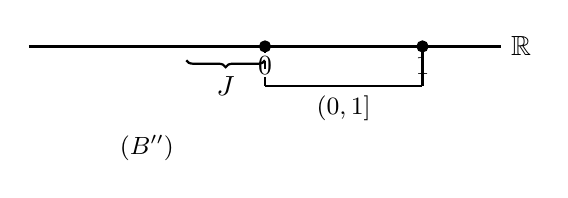
\begin{tikzpicture}

    % Draw the real line
    \draw[thick] (-3,0) -- (3,0);
    
    % Interval J
    \draw[thick, decoration={brace, mirror, raise=5pt}, decorate] (-1,0) -- (0,0) node[midway, below=7pt] {$J$};
    
    % Points on the line
    \filldraw (0,0) circle (2pt) node[below] {$0$};
    \filldraw (2,0) circle (2pt) node[below] {$1$};

    % Bracket for the interval (0,1]
    \draw[thick] (0,-0.5) -- (2,-0.5);
    \draw[thick] (2,-0.5) -- (2,0);
    \draw[dashed] (0,-0.5) -- (0,0);

    % Labeling the interval
    \node[below] at (1,-0.5) {\small $(0,1]$};
    \node[right] at (3,0) {$\mathbb{R}$};

    % Additional notation B''
    \node[below] at (-1.5,-1) {\small $( B'' )$};

\end{tikzpicture}
\end{center}

	   $J$ non è aperto in $\R$ perché  $\forall\varepsilon > 0 \exists$ punti di $\R$, a distanza $< \varepsilon$ da $0$, punti che non sono in $J$.\\
	   Ma  $J$ aperto in $Y$ in topologia di sottospazio perché $Y$ non contiene tali punti\\
	   2) $X = \R$ con topologia euclidea, sia $Y = \Z$ con topologia di sottospazio, Ad esempio  $A = ]-100, 23[\cap Y = \{-99,-98,\ldots,22\}$\\
	   Anche $]-\frac 12, \frac 12[\cap \Z = \{0\}$ è aperto.\\
	   Analogamente\\
	   $]n - \frac {12}, n + \frac 12[\cap \Z = \{n\} \ \ \forall n\in \Z$ è aperto in  $\Z$ in topologia di sottospazio. Quindi la tipologia di sottospazio è discreta.\\
	   3) $X = \R^2$ con topologia euclidea, $Y = \R \times \{0\}$, l'asse  $x.$\\

\begin{center}
\begin{tikzpicture}[scale=1]
    % Draw the x-axis
    \draw[->] (-1,0) -- (2,0) node[right] {$x$};

    % Draw the y-axis
    \draw[->] (0,-1) -- (0,2) node[above] {$y$};

    % Highlight a segment on the x-axis (e.g., [0,1])
    \draw[very thick] (0,0) -- (1,0);

    % Label points
    \fill (0,0) circle (2pt) node[below left] {$0$};
   \fill (1,0) circle (2pt) node[below] {$1$};

    % Indicate open boundary at 1
    \draw (1,0) circle (2pt);
\end{tikzpicture}
\end{center}
	   allora  $A = ]0,1[\times\{0\}$ è aperto in topologia di sottospazio, ad esempio  $B = ]0,1[\times\R$\\
	   %TODO aggiungi immagine 10 marzo 5 47\\
	   \textbf{Osservazione} Verifichiamo che la topologia di sottospazio è una topologia:
	   \[
		   T_Y = \{A\subseteq Y \ | \ \exists B\subseteq X \ \text{ aperto t.c.}  B\cap Y = A\}
	   .\] 
	   Assiomi di topologia
	   \begin{enumerate}
		   \item $\emptyset = \emptyset \cap Y$,  $Y = X\cap Y$
		   \item Siano  $A_i, i\in I$ elemento di  $T_Y$, verifica che  $ \bigcup^{}_{i\in I}A_i$ è in $T_y$\\
			   Scegliamo  $B_i \ \ \forall i\in I$ aperto in  $X$ t.c. \ $ A_i = B_i\cap Y$\\
			    $ \bigcup^{}_{i\in I}A_i = \bigcup^{}_{i\in I}(B_i\cap U) = \bigcup^{}_{i\in I}B_i\cap Y$ dove il primo termine è aperto in X\\
			    da cui $  \bigcup^{}_{i\in I}A_i \in T_Y$.\\
		    \item Siano $A_1, A_2\in T_Y$, scegliamo $B_1,B_2$ aperti in $X$ con $A_i = B_i\cap Y \ \ \forall i\in \{1,2\}$ allora \\
			     $A_1\cap A_2 = (B_1\cap Y)\cap (B_2\cap Y) = B_1\cap B_2)\cap Y$ dove il primo termine è aperto in $X$\\
			     quindi $A_1\cap A_2\in I_y$\\
	   \end{enumerate}
			    \textbf{Osservazione.}\\
		 Sia $C\subseteq Y$ chiuso in topologia di sottospazio. Allora $A = Y\setminus C$ è scrivibile come $A = B\cap Y$ con $B$ aperto in $X$, Allora $D = X\setminus B$ è chiuso in $X, $ e vale $D \cap Y = C$\\
		 Cioè se  $C $ è chiuso in topologia di sottospazio allora esiste $D\subseteq X$ chiuso tale che  $C = D\cap Y$.\\
		 Vale il viceversa se il sottoinsieme  $C$ di $Y$ è scrivibile come  $C = D\cap Y$ con $D \subseteq X$ chiuso, allora  $C$ è chiuso in topologia di sottospazio (esercizio)

% -------------------- Fine Lezione 5 --------------------

\maketitle
	\newpage
	\subsection{boh}
	\textbf{Osservazione:}\\
	Sia $X$ spazio topologico, $Y\subseteq X$ con topologia di sottospazio $T_Y$ .\\
	Considero l'inclusione di $Y$ in $X$ come applicazione

	\begin{center}
		\begin{aligned}
			i : &Y \rightarrow X\\
			    &y \rightarrow y
		\end{aligned}
	\end{center}
	$i$ è costruita (mettendo su $Y$ la topologia $T_Y$). Verifica: sia  $B\subseteq X$ aperto\\
	la controimmagine è $i^{-1}(B)$ Questo è aperto in topologia di sottospazio.\\
	Sia  $T$ una topologia su $Y$ ( non necessariamente = $T_Y$ ), suppongo che $i: Y \rightarrow X $ sia continua anche usando $T$ come topologia su $Y$ \\
	Allora $\forall B\subseteq X$ aperto, $i^{-1}(B)$ è aperto in $Y$ cioè $i^{-1}(B)\in T$. \\
	Al variare di $B$ aperto in $X$, gli insiemi $i^{-1}(B)$ formano  $T_Y$, quindi $T_y \subseteq T$.\\
	Possiamo considerare la famiglia di tutte le topologie su  $Y$ per cui l'inclusione è continua. L'intersezione di esse è contenuta in $T_Y$  perché $ T_Y$ è una di esse, e contiene $T_Y$ perché ogni $T$ siffatta contiene $T_Y$. \\
	Quindi $T_Y$ è la topologia meno fine fra quelle per cui $i$ è continua. 
	\begin{prop}
		Sia $f: X \rightarrow Z$ applicazione continua fra spazi topologici, sia $Y\subseteq X$ con topologia di sottospazio, allora $f|_Y:Y \rightarrow Z$ è continua
	\end{prop}
	\begin{dimo}
		Usiamo l'inclusione $i:X \rightarrow Y$ e osserviamo $f|_Y:Y \rightarrow Z$ concateno con\\
		 \[
			 f\circ i: Y \xrightarrow{i} X \xrightarrow{f} Z
		.\] 
		$f$ e $i$ sono continue, lo è anche $f\circ i$
	\end{dimo}
	\begin{prop}
		Siano $X$ spazio topologico, $Y\subseteq X$ con topologia di sottospazio, $Z$ spazio topologico e $f : Z \rightarrow Y$.\\
		Consideriamo l'estensione del codominio di $f$ da $Y$ a $X$ che è l'applicazione  $i\circ f :Z\xrightarrow{f} Y \xrightarrow{i} X$\\
		Allora $f$ è continua se e solo se $i\circ f$ è continua.
	\end{prop}
	\begin{dimo}
		%TODO disegno 11 marzo 5:44
		$ ( \Rightarrow )$ ovvio poiché $i\circ f$ è composizione di applicazioni continue\\
		$ ( \Leftarrow)$ Sia $A\subseteq Y$ aperto, scegliamo $B\subseteq X$ aperto tale che $B\cap Y = A$.\\
		Allora  $f^{-1}(A) = (i\circ f)^{-1}(B)$ \\
		poiché chiedere che $z\in Z$ vada in $A$ tramite $f$ è equivalente a richiedere che vada in $B$.\\
		Allora $f^{-1}(A)$ è aperto per continuità di $i\circ f$
	\end{dimo}
	\textbf{Osservazione}\\
	Data in generale $f: Z \rightarrow X$ spesso la si restringe all'immagine
	\begin{center}
		\begin{aligned}
			\tilde f: &Z \rightarrow Im(f)\\
				  & z - f(z)
		\end{aligned}
	\end{center}
	vale $f$ continua  $ \Leftrightarrow \tilde f$ continua, perché posso considerare l'inclusione 
	\[
	 i: Im(f) \rightarrow X
	.\]  
	e allora $f = i \circ \tilde f$\\
	 \textbf{Esempio:}\\
	 $X = \R$ con topologia euclidea.\\
	 $Y = [0,1[$ con topologia di sottospazio
	 \[
	  Z = ]0,1[ \ \ (\subseteq Y)
	 .\] 
	 Sia verifica facilmente (esercizio) che la chiusura di $Z$ in $Y$ è $[0,1[$e la chiusura di $Z$ in $X$ è $[0,1]$ \\
	 Le chiusure sono diverse, ma
	 \[
	  [0,1[ = [0,1]\cap Y
	 .\] 
	 dove il primo intervallo è in $Y$ e il secondo intervallo in $X$\\
	 Questo si generalizza.
	 \begin{lemm}
	 	Sia $X$ spazio topologico, $Y\subseteq X$ con topologia di sottospazio, $Z\subseteq Y$ la chiusura di $Z$ in $Y$ è uguale a $Y$ intersecato la chiusura di $Z$ in $X$
	 \end{lemm}
	 \begin{dimo}
		 Chiusura di $Z $ in $Y = \displaystyle \bigcap_{\substack{C\subseteq Y,\\ C\text{ chiuso in } Y,\\ C\supseteq Z}}C = \ldots $ \\
		 Per ogni tale $C$ scelgo un $D\subseteq X$ chiuso in $X$ tale che $C = D\cap Y$\\
		  \[
			  \ldots = \bigcap_{\substack{C\subset U,\\ C\text{ chiuso in } Y,\\ C\supseteq Z,\\ D\subseteq X,\\ D \text{ chiuso in } X \\ t.c. \ D\cap Y = C}}D\cap Y 
		 .\] 
		 \[
			 = \bigcap_{\substack{D'\subseteq X,\\ D'\text{ chiuso in } X,\\ D'\supset Z}}D'\cap Y
		 .\] 
		 L'ultima uguaglianza vale perché ogni $D$ della prima intersezione compare fra i $D$ della seconda intersezione, Per ogni $D'$ della seconda seconda intersezione considero $C = D'\cap Y$ che è in  $Y$, chiuso in $Y$, contenente $Z$, quindi compare fra i  $C$ della prima intersezione; ad esso corrisponde un $D$ della prima intersezione, che soddisfa $D\cap Y = C =D'\cap Y.$\\
		 Quindi per ogni  $D'$ della seconda intersezione esiste un $D$ della prima con la stessa intersezione con $Y$, ovvero  $D\cap Y = D'\cap Y$, Quindi vale l'uguaglianza.\\
		 L'uguaglianza prosegue:\\
		  \[
			  = \left( \bigcap_{\substack{D'\subsetteq Z,\\ D'\text{ chiuso in } X,\\ D'\supseteq Z}} D' \right)\cap Y
		 .\] 
		 dove la parentesi è la chiusura di $Z$ in $X$
	 \end{dimo}
	 \textbf{Osservazione}\\
	 Attenzione: non vale un enunciato analogo con la parte interna.\\
	 Ad esempio $X = \R$ cn topologia euclidea $Y = \Z$  $Z= \{0\}$\\
	 La parte interna di  $Z$ in $X$ è vuota, perché $Z$ non contiene alcun aperto di $\R$\\
	 Invece la topologia di sottospazio su  $Y$ è la topologia discreta e $Z$ è aperto in $Y$.\\
	 Quindi  $Z$ è la propria parte interna come sottoinsieme di $Y$.
	 \begin{defi}
	 	Sia $f: X \Rightarrow Y $ un'applicazione continua fra spazi topologici, $f$ è un'inversione topologica se la restrizione
		\begin{center}
			\begin{aligned}
				\tilde f: &X \rightarrow f(X)\\
					  &x \rightarrow f(x)
			\end{aligned}
		\end{center}
		è un omeomorfismo, dove su $f(X)\subseteq Y$ metto la topologia di sottospazio.
	 \end{defi}
	 \textbf{Esempio}\\
	 1) Considero 
	 \begin{center}
	 	\begin{aligned}
			&\R \rightarrow \R \\
			&x \rightarrow (x,0)
	 	\end{aligned}
	 \end{center}
	 (qui $\R, \R^2$con topologia euclidea) è un immersione, la verifica è per esercizio.\\
	 2) 
	 \begin{center}
	 	\begin{aligned}
			$f : $&$[0,2\pi[ \rightarrow \C$\\
			   & $t \rightarrow e^{it}$
	 	\end{aligned}
	 \end{center}
	 Su $[0,2\pi[\subseteq \R$\\
	 metto la topologia di sottospazio indotta dalla topologia euclidea su  $\R,$ su $\C = \R^2$ metto la topologia euclidea\\
	 È continua, iniettiva e $f([0,2\pi[) = S^1 = \{z\in\C \ | \ |z|=1\}$\\
	 Questa  $f$ non è un'immersione, infatti $[0,\pi[$ è aperto nel dominio, ma $f([0,2[)$ non è aperto in $S_1$ con topologia di sottospazio.
	 %TODO aggiungi figura 6:40
	 quel chiuso dovrebbe essere interesezione tra la circonferenza e un aperto di $\R^2$, Ciò non è possibile perchè ci sarebbe un intorno su un estremo della circonferenza.\\
	 \subsection{Prodotti topologici}
	 Siano $P,Q$ spazi topologici.\\
	 vogliamo definire una topologia "naturale" su $P\times Q$.\\
	  \textbf{Esempio:}\\
Considero $P = Q = \R$ con topologia euclidea
 \[
 P\times Q = \R\times \R = \R^2
.\] 
La topologia su $\R^2$ sarà quella euclidea. Considero ad esempio
\[
	U \subseteq \R\text{ aperto}, \ \ V\subseteq\R\text{ aperto}
.\] 
il prodotto $U\times V$ sarà aperto in  $\R^2$, posso pensare che questa sia quindi la mia topologia, ma vediamo qualche esempio con la topologia euclidea.\\
Ad esempio  $U = ]a,b[ \ \ \ V = ]c,d[$, allora  $U\itimes V = ]a,b[\times]c,d[$ è un rettangolo aperto\\
Anche un disco aperto in  $\R^2$ è aperto in topologia euclidea, ma non riesco a scriverlo con questo prodotto  $U\times V$ con $U\subseteq \R, \ V\subseteq \R$\\
Potrei prendere
 \[
	 B = \{U\times V \ | \ \ \substack{U\subseteq \R \text{ aperto },\\ \hspace{-3px}V\subseteq\R\text{ aperto }}\}
.\] 
come base per la topologia su $\R\times\R$
 \begin{defi}
	Siano $P,Q$ spazi topologici, la topologia prodotto su $P\times Q$ è la meno fine fra quelle per cui le proiezioni:
	\begin{center}
		\begin{aligned}
			p:& P\times Q \rightarrow P\\
			  &(a,b) \rightarrow a\\
			q:&P\times Q \rightarrow Q\\
			  &(a,b) \rightarrow b
		\end{aligned}
	\end{center}
	Sono continue.
\end{defi}
\textbf{Osservazione}\\
Esistono topologie su $P\times Q$ tali che  $p$ e $q$ sono continue, per esempio la topologia discreta su $P\times Q$\\
La topologia prodotto è l'intersezione di tutte le topologia per cui  $p$ e $q$ sono continue.
\begin{teo}
	
\end{teo}

% -------------------- Fine Lezione 6 --------------------

\end{document}
